\documentclass[letterpaper,10pt]{article}

\usepackage{titling}
\usepackage{listings}
\usepackage{url}
\usepackage{setspace}
\usepackage{subfig}
\usepackage{sectsty}
\usepackage{pdfpages}
\usepackage{colortbl}
\usepackage{multirow}
\usepackage{relsize}
\usepackage{amsmath}
\usepackage{fancyvrb}
\usepackage{amsmath,amssymb,amsthm,graphicx,xspace}
\usepackage[titlenotnumbered,noend,noline]{algorithm2e}
\usepackage[compact]{titlesec}
\usepackage[default]{droidserif}
\usepackage[T1]{fontenc}
\usepackage{tikz}
\usetikzlibrary{arrows,automata,shapes,trees,matrix,chains,scopes,positioning,calc}
\tikzstyle{block} = [rectangle, draw, fill=blue!20, 
    text width=2.5em, text centered, rounded corners, minimum height=2em]
\tikzstyle{bw} = [rectangle, draw, fill=blue!20, 
    text width=4em, text centered, rounded corners, minimum height=2em]

\definecolor{namerow}{cmyk}{.40,.40,.40,.40}
\definecolor{namecol}{cmyk}{.40,.40,.40,.40}

\let\LaTeXtitle\title
\renewcommand{\title}[1]{\LaTeXtitle{\textsf{#1}}}


\newcommand{\handout}[5]{
  \noindent
  \begin{center}
  \framebox{
    \vbox{
      \hbox to 5.78in { {\bf ECE155: Engineering Design with Embedded Systems } \hfill #2 }
      \vspace{4mm}
      \hbox to 5.78in { {\Large \hfill #4  \hfill} }
      \vspace{2mm}
      \hbox to 5.78in { {\em #3 \hfill} }
    }
  }
  \end{center}
  \vspace*{4mm}
}

\newcommand{\lecture}[3]{\handout{#1}{#2}{#3}{Lecture #1}}
\newcommand{\tuple}[1]{\ensuremath{\left\langle #1 \right\rangle}\xspace}

\addtolength{\oddsidemargin}{-1.000in}
\addtolength{\evensidemargin}{-0.500in}
\addtolength{\textwidth}{2.0in}
\addtolength{\topmargin}{-1.000in}
\addtolength{\textheight}{1.75in}
\addtolength{\parskip}{\baselineskip}
\setlength{\parindent}{0in}
\renewcommand{\baselinestretch}{1.5}
\newcommand{\term}{Spring 2014}

\singlespace


\begin{document}

\lecture{ 28 --- Interval \& Watchdog Timers}{\term}{Patrick Lam}

Previously, we've discussed the idea of polling vs. interrupts. In this lecture, we'll talk about how to use a timer, and its relationship to polling and other embedded
systems concepts.

\section*{Timers}
Recall that in \emph{periodic polling}, the software polls a device at
fixed intervals. The usual way of implementing periodic polling is
through timers. Two potential applications of timers:
\begin{itemize}
\item perform a task occasionally (e.g. raising alarms, or polling); or
\item reset a system that's gotten stuck.
\end{itemize}




\paragraph{Skill.} In today's lecture, you'll learn how to use Java timers to
implement interval timers and watchdog timers. You'll also learn about
the difference between Android timers and Java timers.

\subsection*{Interval Timers.} Interval timers are appropriate for recurring tasks. 
For instance, one could implement light sensor polling with an
interval timer (but you don't need to do this in Android, since the
system sends you events when the value changes). We've seen the use of
{\tt Handler} to implement interval timers, which performs tasks
occasionally.  You can always use more than one timer at a time, each
with different frequencies.

Reminder: Here's some code for executing an infinitely recurring task using
{\tt Handler}:

{\small \begin{lstlisting}
  Handler h = new Handler();
  Runnable r = new Runnable() {
    public void run() {
      // execute the task
      h.postDelayed(this, delayInMS);
    }
  };
  h.postDelayed(r, delayInMS);
\end{lstlisting}}

By the way, you can cancel an upcoming task like this:
{\small \begin{lstlisting}
  h.removeCallbacks(r);
\end{lstlisting}}

\paragraph{True Interval Timers.}
Strictly speaking, the timers we'll be implementing aren't actually
interval timers. A true interval timer interrupts the processor,
rather than waiting for the executing thread to become free.

We can simulate an interval timer more closely using the {\tt Timer}
class~\cite{ody}. Such a timer executes in a different thread,
so it doesn't need to wait for processor availability. A serious
problem is that other threads can't do updates to the user interface
(UI). Timers have more overhead and generally aren't the right thing
on Android, but you should know about them.

Here's how you can use {\tt Timer} successfully. You can put this code
anywhere, including {\tt onCreate()} or in an on-click listener.

{\small \begin{lstlisting}
  Timer t = new Timer();
  t.schedule(new TimerTask() {
    @Override
    public void run() {
      runOnUiThread(timerTick);
    }
  }, firstDelayMS, repeatIntervalMS);
\end{lstlisting}}

You are creating a Java {\tt Timer} object, which takes a
delay-before-first-event and a repeat interval, both in
milliseconds. If you omit the repeat interval, the {\tt Timer} only
fires once. In the {\tt run()} method of the {\tt TimerTask} (again,
event-oriented programming), you are asking Android to run the {\tt
  timerTick} {\tt Runnable} on the UI thread. If you just call {\tt
  timerTick.run()}, your app will crash!

Let's also create the {\tt timerTick} object.
{\small \begin{lstlisting}
  Runnable timerTick = new Runnable() {
    @Override
    public void run() {
      Toast.makeText(getApplicationContext(), 
                     "ding!", Toast.LENGTH_SHORT).show();
    }
  };
\end{lstlisting}}

A recap: you have to do the following to set up a Java timer.
\begin{itemize}
\item instantiate a new {\tt Timer} object;
\item schedule a {\tt TimerTask} on that {\tt Timer};
\item inside the {\tt TimerTask}, invoke a {\tt Runnable} to run on the
UI thread; and
\item implement the {\tt run()} method on the {\tt Runnable} to effect
  UI changes.  
\end{itemize}

\subsection*{Watchdog Timers} The other timer application I mentioned
is that of a watchdog timer, which can observe that a system appears to
be stuck and take some action.

Watchdog timers are commonly found in computer systems where humans cannot easily take corrective action. If a NASA satellite gets stuck somehow, NASA usually cannot send astronauts up to press the reset button. If not for the ability to automatically restart, the satellite would be permanently disabled.

When a watchdog timer is set up, the system needs to indicate, before the limit of the timer, that everything is okay. If the system thinks all is well, either by checking some fault conditions or simply by default, the watchdog timer is reset. 

An example of a potential fault condition is checking if free memory is below a reference value, such as 256~MB. If the system detects free memory is above 256~MB then then it resets the watchdog timer. If it is below 256~MB, then the watchdog timer is not reset and the timer will fire, taking some corrective action (i.e., freeing up some memory).

Corrective action is variable, based on the system the watchdog is looking after. In some cases, corrective action is minor (killing a task), but in physical systems it might be necessary to turn off motors for safety. 

\paragraph{Implementing Watchdogs with Interval Timers.}
You can build a watchdog timer using an interval timer.
\begin{itemize}
\item Set the timer interval to be the largest allowable time for a task
to take. Start the timer.
\item If the timer fires, the task took too long.
\item The timer event handler should still execute, so it can deal with
the situation (for instance, by killing the task.)
\end{itemize}

{\sf Why wouldn't the event handler execute?}\\[2em]

When designing an embedded system, you might use specialized hardware
for a watchdog timer. This gives it some resilience to failures in the
rest of the system. The fact that {\tt Timer}s run in separate threads
also give them some resilience.

Choosing an appropriate timer length is important and is usually a matter of practice and experience. Choosing a length that is too short means the system will get reset even when nothing is really wrong; in the extreme case, no meaningful work is accomplished because the system is always being interrupted. Choosing an interval that is too long can result in the system being stuck for a long period of time before corrective action is taken; in the extreme case, the corrective action does not happen in time and the system suffers a serious failure.

\paragraph{Example.}
Here's an example of an Android analogy of a watchdog timer.

{\scriptsize \begin{lstlisting}
class MainActivity extends Activity
{
    @Override
    public void onCreate(Bundle savedInstanceState) {
	super.onCreate(savedInstanceState);
	setContentView(R.layout.activity_main);

        final Timer watchdogTimer = new Timer();

        // When this task is run, finish the activity.
        final Runnable timerTick = new Runnable() {
          @Override 
          public void run() {
            MainActivity.this.finish();
          }
        };

        // User has 10 seconds to complete this page, otherwise finish.
        watchdogTimer.schedule(new TimerTask() {
          @Override
          public void run() {
            runOnUiThread(timerTick);
          }
        }, 10000);

        Button b = (Button) findViewById(R.id.next_page);
	b.setOnClickListener(new View.OnClickListener() {
	  @Override
	  public void onClick(View arg0) {
            watchdogTimer.cancel();
            Intent browserIntent = new Intent(Intent.ACTION_VIEW);
	    browserIntent.setData(Uri.parse("http://www.patricklam.ca"));
	    startActivity(browserIntent);
          }
        });
    }
}
\end{lstlisting}}

If the user clicks on the button fast enough,
the app navigates to \texttt{patricklam.ca}. Otherwise, the app's main activity finishes.

\paragraph{Multiple-Stage Watchdog Timers.}
So far we have only discussed corrective action as if it is all-or-nothing. However, watchdog timers can have multiple stages -- multiple levels of response. If the first level of response does not resolve the problem, then a second level of response will activate to take more drastic action. 

Suppose there is a system with a two-stage watchdog timer. Under normal operation, the first stage timer is reset regularly. If this timer is not reset, then stage one activates: it sets up a watchdog timer for stage two and attempts to take corrective action. If stage one's corrective action succeeds, it cancels stage two's activation. Otherwise, stage two activates and takes some more serious action.

Example: the software has a two-stage watchdog timer. The first watchdog timer attempts to restart the application \texttt{example.exe}. The first level has a timer length of 180 seconds; every 60 seconds, \texttt{example.exe} resets the watchdog timer. If the reset doesn't happen, the watchdog activates. Its first step is to start another watchdog timer, with a length of 120 seconds. Then the first watchdog tries to restart \texttt{example.exe}. If the first watchdog does not successfully restart the program within the 120 seconds, the second watchdog timer activates and restarts the computer.

\subsection*{Timer Coalescing}

Using timers has an impact on power consumption in an embedded or mobile system (phones, laptops, et cetera). Suppose we have a phone with an interval timer set up with an interval of 1000ms. Then every second the system will execute the timer's action -- the system wakes up, runs the action, then goes back to sleep. This is okay, but if we have multiple concurrent interval timers then the system might never actually get to sleep, because it is constantly being woken up by interval timers that are just slightly out of sync with one another. See the example below:

\begin{center}
	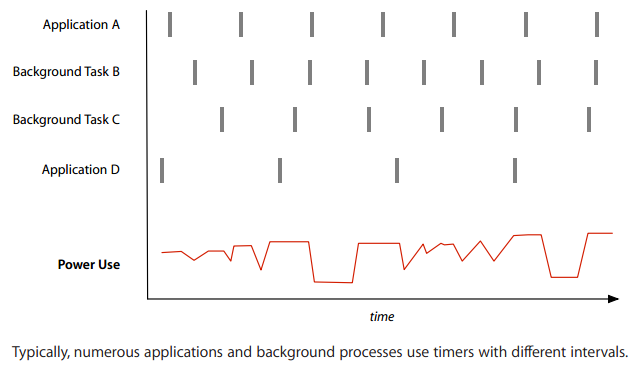
\includegraphics[width=0.7\textwidth]{images/coalesced_before.png}
	\cite{coalesce}
\end{center}

There is a way to deal with this, and it hinges on a critical point about timers. When a timer is set up for a specific time, such as 1000 ms, the system does not promise that the timer will run exactly 1000 ms from now. What it really says is that the timer task will execute \textit{no sooner than} 1000 ms from now. It might happen that the task runs 1000 ms from now, but it could be 1004 ms or 1200 ms later, yet it could not be 997 ms or 980 ms later.

This allows operating systems to do something clever to deal with the problem of timers that are close together but not exactly. It can delay some of them a little bit so that they line up. See the updated example:

\begin{center}
	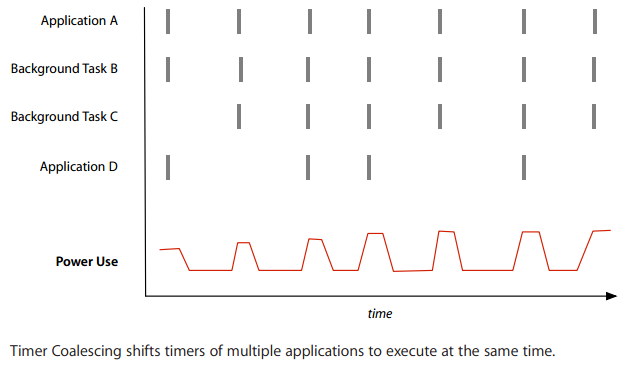
\includegraphics[width=0.7\textwidth]{images/coalesced-after.png}
	\cite{coalesce}
\end{center}

Now, this image is not a hundred percent accurate. A careful examination shows that some of the lines were moved to the left (back in time) to make them line up and that would violate the no-sooner-than semantics. This is just artistic license to make the graphic look a little bit nicer (blame the authors,~\cite{coalesce}), but in reality the lines could only be shifted to the right.

Despite that, the image shows clearly the impact of timer coalescing on power consumption. Most modern operating systems do this, including Windows and Mac OS X.

\bibliographystyle{alpha}
\bibliography{155}



\end{document}
